\nhom{G. Bài dữ liệu và mô phỏng: lời giải đã chạy}
\noindent Kết quả dưới đây được tính từ dữ liệu lưu kèm và mã
\texttt{kde\_computation/run\_kde\_experiments.py}, seed $20260930$.
Các bảng được sinh tự động từ output; đồ thị là kết quả tính toán, không phải hình minh họa giả định.
Quy ước: $s$ dùng mẫu số $n-1$; phân vị nội suy tuyến tính; tích phân số dùng quy tắc hình thang.

\begin{problem}[KDE-41. W6.5--6.7: CEO, glass, CV, các dạng nhân và băng tin cậy.]\label{k:41}
\textit{(Nguồn: W6.5--6.7, tr.143.)} Ước lượng mật độ bằng histogram và KDE; chọn mức làm trơn bằng least-squares CV, so với normal reference; thay đổi bandwidth và dạng nhân; dùng băng tin cậy để đánh giá các bướu.
\end{problem}
\begin{solution}
\textbf{1. Dữ liệu và những chi tiết làm thay đổi đáp số.}
CEO: bản lưu \texttt{GLMsData::ceo} từ nguồn DASL/Forbes 1993, cùng bộ 60 công ty được nêu trong đề. Có một lương bị thiếu: bỏ riêng giá trị thiếu, \emph{không thay bằng 0}, nên $n=59$. Đơn vị là nghìn USD; min $21$, max $1103$.
Nguồn định nghĩa biến: \href{https://search.r-project.org/CRAN/refmans/GLMsData/html/ceo.html}{tài liệu gói GLMsData}; \href{https://ics.uci.edu/~jutts/8/readme.html}{tài liệu Utts--Heckard tại UCI} xác nhận đúng liên kết DASL của đề và một giá trị thiếu.

Glass: lấy trực tiếp \href{https://stat.cmu.edu/~larry/all-of-nonpar/=data/glass.dat}{file trên trang Wasserman}, $214$ dòng. Cột đầu trong nội dung là chỉ số dòng, sau đó mới đến biến \texttt{RI}. Phân tích \texttt{RI}, không phân tích chỉ số dòng. Biến trong sách đã đổi thang:
\[
 Z=1000(\mathrm{RI}_{\rm original}-1.518),\qquad
 h_{\rm original}=h_Z/1000.
\]
Nếu cần mật độ trên thang gốc thì $\widehat f_{\mathrm{RI}}(r)=1000\widehat f_Z(1000(r-1.518))$.
Ví dụ giá trị đầu là $3.01$, ứng với RI gốc $1.52101$; min, max của $Z$ là $-6.85,15.93$.

\textbf{2. Tính bandwidth và histogram.}
Tính $h_{NR}=1.06\min(s,\mathrm{IQR}/1.34)n^{-1/5}$.
Tìm $h_{CV}$ trên 101 điểm cách đều theo log trong $[0.06h_{NR},4h_{NR}]$ bằng \emph{công thức chính xác}
\[
 \widehat J(h)=\frac{1}{n^2h}\sum_{i,j}\phi_{\sqrt2}\!\left(\frac{X_i-X_j}{h}\right)
 -\frac{2}{n(n-1)h}\sum_{i\ne j}\phi\!\left(\frac{X_i-X_j}{h}\right).
\]
$\phi_{\sqrt2}$ là mật độ $N(0,2)$, không phải $\phi$.
Đáp số là cực tiểu \emph{trên lưới đã công bố}; không gọi là nghiệm tối ưu liên tục chính xác.
Cả hai nghiệm nằm bên trong lưới.

Histogram dùng miền cố định $[0,1400]$ cho CEO và $[-8,18]$ cho glass; với mỗi $k=4,\ldots,45$, chia thành $k$ bin đều, $\Delta=(b-a)/k$, rồi cực tiểu
\[
 \widehat J_{\rm hist}(k)=\frac{2}{(n-1)\Delta}
 -\frac{n+1}{(n-1)\Delta}\sum_j(N_j/n)^2.
\]
Giữ cùng gốc bin khi so sánh: đổi cả gốc bin có thể đổi histogram và đáp số CV.
\begin{center}\begin{tabular}{lrr}\toprule Đại lượng & CEO & Glass\\\midrule
$n$ & 59 & 214\\
Trung bình & 404.17 & 0.36542\\
$s$ & 220.53 & 3.0369\\
IQR & 289.5 & 2.635\\
$h_{NR}$ & 101.32 & 0.71269\\
$h_{CV}$ & 69.454 & 0.23925\\
Số bin histogram CV & 7 & 31\\
Độ rộng bin & 200 & 0.83871\\
Ngưỡng băng đồng thời & 3.1685 & 3.5177\\
\bottomrule\end{tabular}\end{center}
Ví dụ CEO: $\widehat\sigma=\min(220.5335,289.5/1.34)=216.0448$, nên $h_{NR}=101.3163$; $h_{CV}=69.4540$ cho đường ít trơn hơn.
Glass có $h_{CV}/h_{NR}\approx0.336$, nên CV để lộ nhiều cấu trúc nhỏ hơn normal reference.
CV âm là bình thường vì nó ước lượng MISE trừ $R(f)$.

\textbf{3. So sánh dạng nhân một cách công bằng.}
Vẽ Gaussian, Epanechnikov và đều với $h_K\sqrt{\mu_2(K)}=h_{CV}$, tức bandwidth lần lượt là $h_{CV},\sqrt5h_{CV},\sqrt3h_{CV}$.
Như vậy các nhân có cùng phương sai làm trơn; dùng cùng một con số $h$ cho cả ba sẽ trộn lẫn hiệu ứng dạng nhân với độ rộng nhân.
Đồ thị cho thấy hình dạng tổng thể gần nhau, nhưng nhân đều có bước nhảy và các nhân compact vẫn khác ở những bướu nhỏ. Không khẳng định ba đường phải trùng nhau trong mẫu hữu hạn.
\begin{center}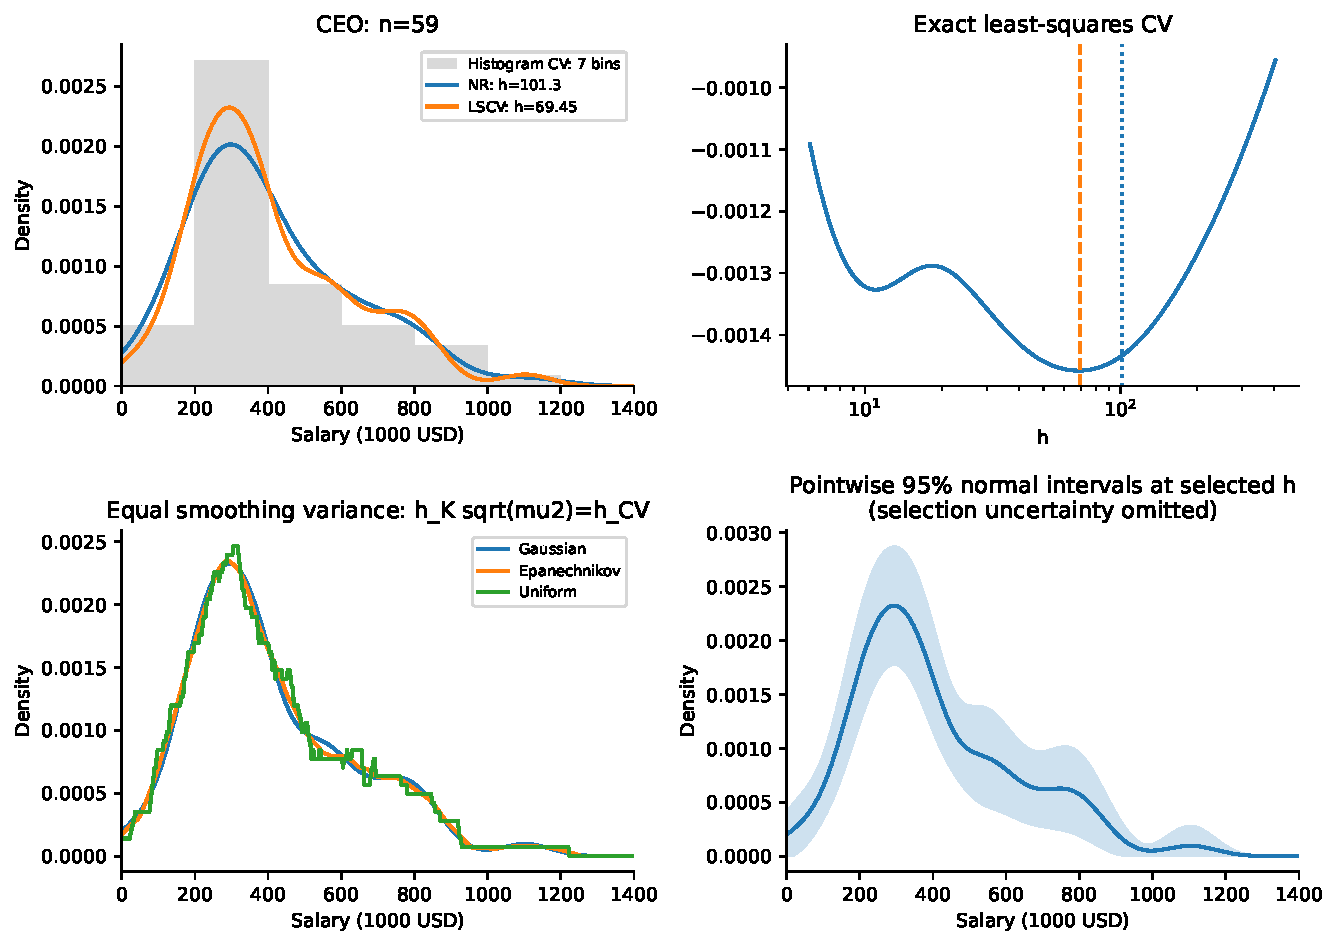
\includegraphics[width=\linewidth]{kde_computation/figures/ceo_overview.pdf}\end{center}
\begin{center}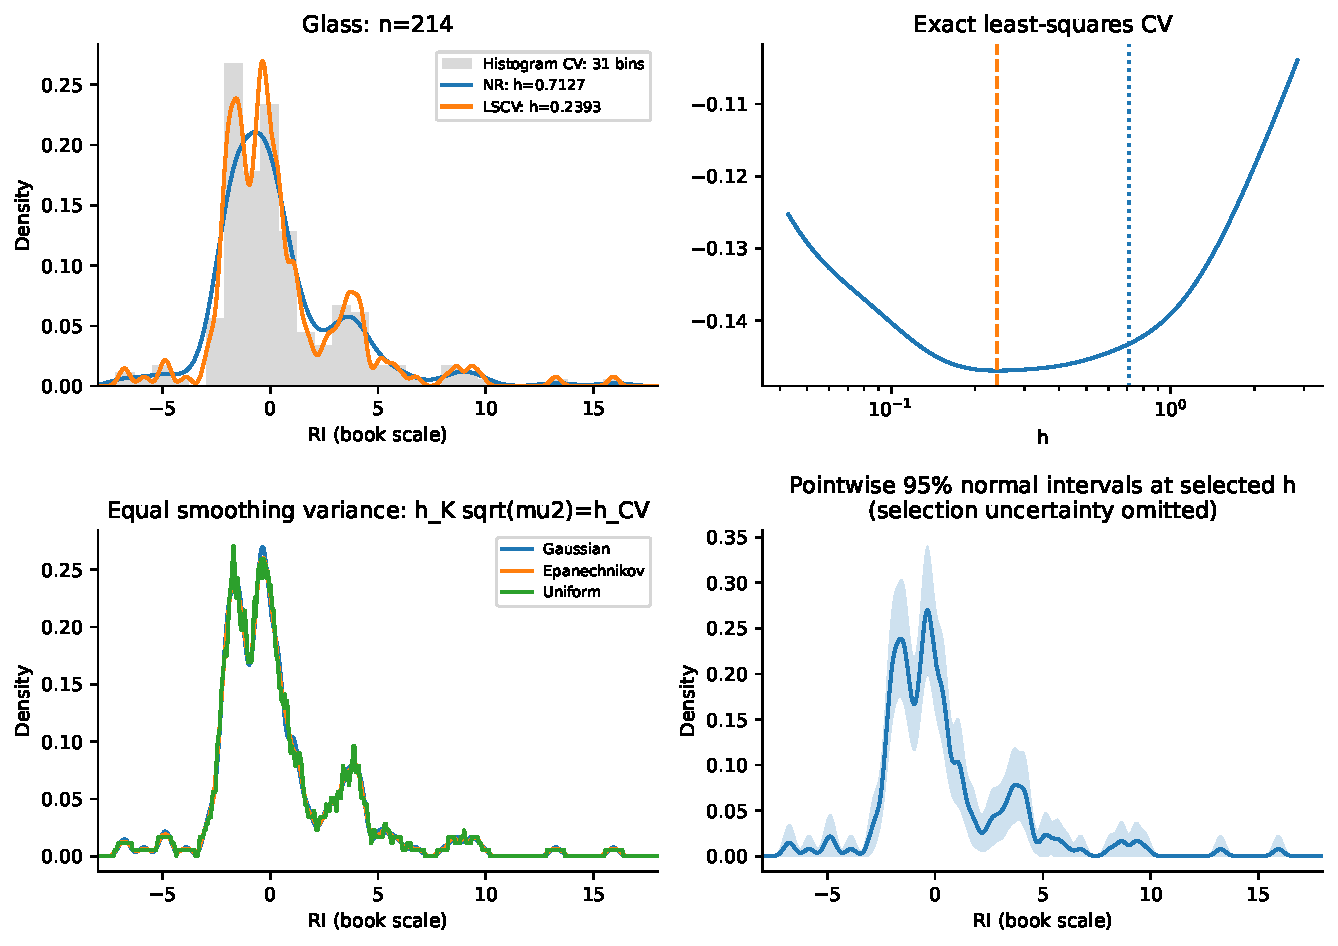
\includegraphics[width=\linewidth]{kde_computation/figures/glass_overview.pdf}\end{center}

\textbf{4. Khoảng từng điểm khác băng đồng thời.}
Đặt $W_i(x,h)=h^{-1}\phi((x-X_i)/h)$ và $\overline W=\widehat f_h(x)$. Sai số chuẩn thực nghiệm là
\[
 \widehat{\se}_h(x)=\sqrt{\frac{\sum_i(W_i-\overline W)^2}{n(n-1)}}.
\]
Khoảng $\widehat f_h\pm1.96\widehat{\se}_h$ là khoảng chuẩn xấp xỉ \emph{từng điểm} cho $f_h=\E\widehat f_h$ nếu $h$ cố định. Các hình overview vẽ khoảng này ở $h_{CV}$ chỉ để minh họa biến thiên; chúng chưa tính bất định do chọn $h$, không phải một băng 95\% được bảo đảm cho $f$.

Để khảo sát nhiều $h$, dùng họ định trước
\[
 H_{CEO}=\{40,80,120,160,240\},\qquad
 H_{glass}=\{0.2,0.4,0.8,1.6,3.2\},
\]
và 241 điểm đều trên mỗi miền vẽ. Sinh $1999$ vector $\xi^{(b)}\sim N(0,I_n)$, tính
\[
 T_b=\max_{h\in H,\,x\in G}
 \left|\frac{\sum_i\xi_i^{(b)}(W_i(x,h)-\overline W(x,h))}
 {\sqrt{\sum_i(W_i(x,h)-\overline W(x,h))^2}}\right|.
\]
Lấy $c_{.95}$ là phân vị thực nghiệm 95\% của $T_b$, được $3.1685$ cho CEO và $3.5177$ cho glass. Băng là
\[
 [\max(0,\widehat f_h-c_{.95}\widehat{\se}_h),\;
 \widehat f_h+c_{.95}\widehat{\se}_h].
\]
Đây là băng multiplier \emph{xấp xỉ}, đồng thời trên họ hữu hạn $(x,h)$, cho các mật độ đã làm trơn $f_h$. Không suy ra bao phủ mọi $x\in\R$, không có bảo đảm hữu hạn mẫu 95\% và không loại bỏ bias đối với $f$.
Để tránh diễn giải đuôi quá ít dữ liệu, chỉ tô băng ở điểm có
$n_{\rm eff}=(\sum_i W_i)^2/\sum_iW_i^2\ge5$; ngưỡng này là quy tắc hiển thị, không phải định lý bảo đảm xấp xỉ chuẩn.

\textbf{5. Băng cho histogram, kể cả sau khi chọn số bin.}
Với bin cố định, $N_j\sim\operatorname{Binomial}(n,p_j)$. Có tổng cộng
$M=\sum_{k=4}^{45}k=1029$ bin trong tất cả các phép chia đang xét. Đặt $\eta=0.05/(2M)$; dùng Clopper--Pearson:
\[
 L_j=B^{-1}_{N_j,n-N_j+1}(\eta),\qquad
 U_j=B^{-1}_{N_j+1,n-N_j}(1-\eta),
\]
quy ước $L_j=0$ nếu $N_j=0$, $U_j=1$ nếu $N_j=n$.
Theo union bound, xác suất tất cả $p_j\in[L_j,U_j]$ ít nhất 95\%, không cần các bin độc lập. Do đó vẫn được chọn $k$ bằng CV trong họ này.
Băng mật độ $[L_j/\Delta,U_j/\Delta]$ bao phủ \emph{trung bình mật độ trên bin} $p_j/\Delta$, không phải từng $f(x)$ trong bin.
Hình dưới so sánh số bin nhỏ hơn, bằng và lớn hơn nghiệm CV. Băng rộng là hệ quả của bảo vệ đồng thời cả họ, không phải lỗi vẽ.
\begin{center}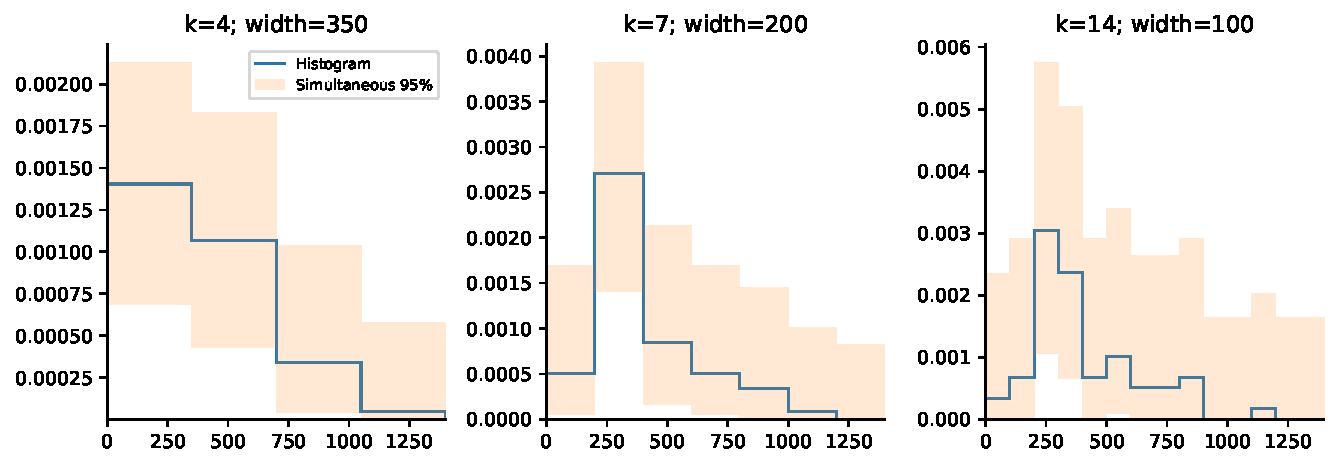
\includegraphics[width=\linewidth]{kde_computation/figures/ceo_histograms.pdf}\end{center}
\begin{center}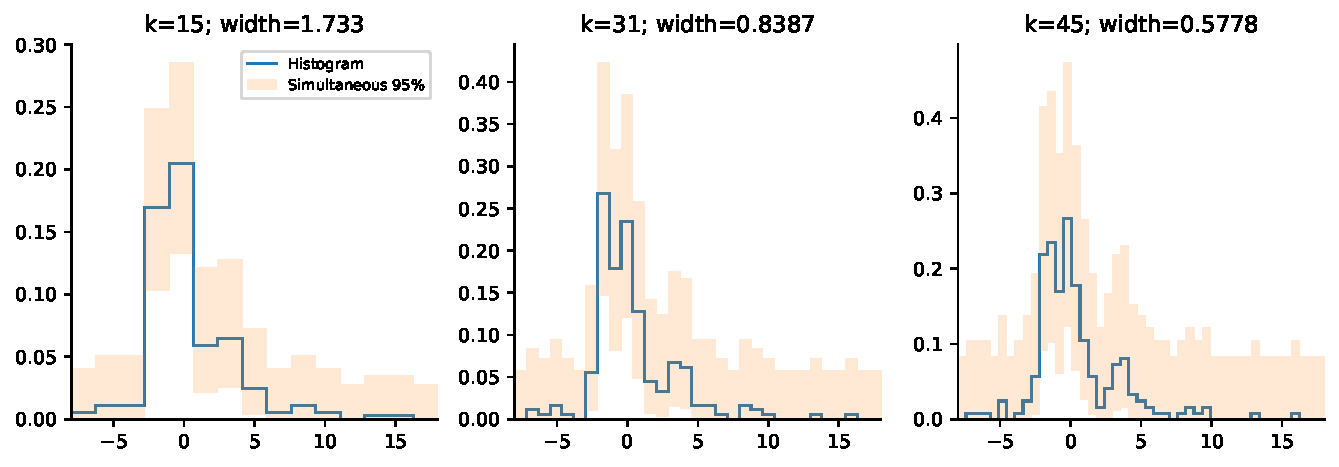
\includegraphics[width=\linewidth]{kde_computation/figures/glass_histograms.pdf}\end{center}

\textbf{6. Các bướu có thật không? Cách trả lời từ kết quả.}
CEO: trên lưới vẽ, KDE với $h=40$ có năm cực đại cục bộ, gần $52.5,291.7,542.5,775.8,1102.5$; tăng lên $h=120$ chỉ còn một cực đại gần $303.3$. Các bướu nhỏ phụ thuộc mạnh vào bandwidth. Để kiểm tra chứ không chỉ nhìn hình, áp dụng cùng thuật toán multiplier cho
\[
 W_i'(x,h)=-\frac{x-X_i}{h^3}\phi((x-X_i)/h),
\]
nhắm đạo hàm $f_h'$. Màu đỏ: băng đạo hàm nằm trên 0; xanh: nằm dưới 0; trắng: chưa xác định dấu hoặc quá ít dữ liệu. Băng đạo hàm dùng một hiệu chỉnh riêng cho toàn họ, không đồng thời 95\% với băng mật độ.
Ở $h=40$, không điểm nào của CEO có dấu đạo hàm được xác định theo tiêu chuẩn này. Vì vậy chưa đủ bằng chứng để diễn giải năm bướu thành năm nhóm lương thật. \emph{Không đủ bằng chứng nhiều mode không đồng nghĩa chứng minh mật độ một mode.}

Glass: ở $h=0.2$ có nhiều gợn; ở $h=1.6$ và $3.2$ chỉ còn một đỉnh lớn quanh vùng RI đổi thang âm nhẹ. Bản đồ đạo hàm tại $h=0.2$ cũng không xác định được dấu ở điểm nào; ở $h=0.4$ chỉ có một số điểm tăng được xác định, chưa xác định điểm giảm. Những gợn nhỏ vì thế chưa được xác nhận bằng phân tích này. Ở thang lớn hơn, xu hướng tăng rồi giảm của khối chính rõ hơn.
Đây là khảo sát đạo hàm trên lưới theo tinh thần scale-space; không gọi là triển khai đầy đủ SiZer của Chaudhuri--Marron.
\begin{center}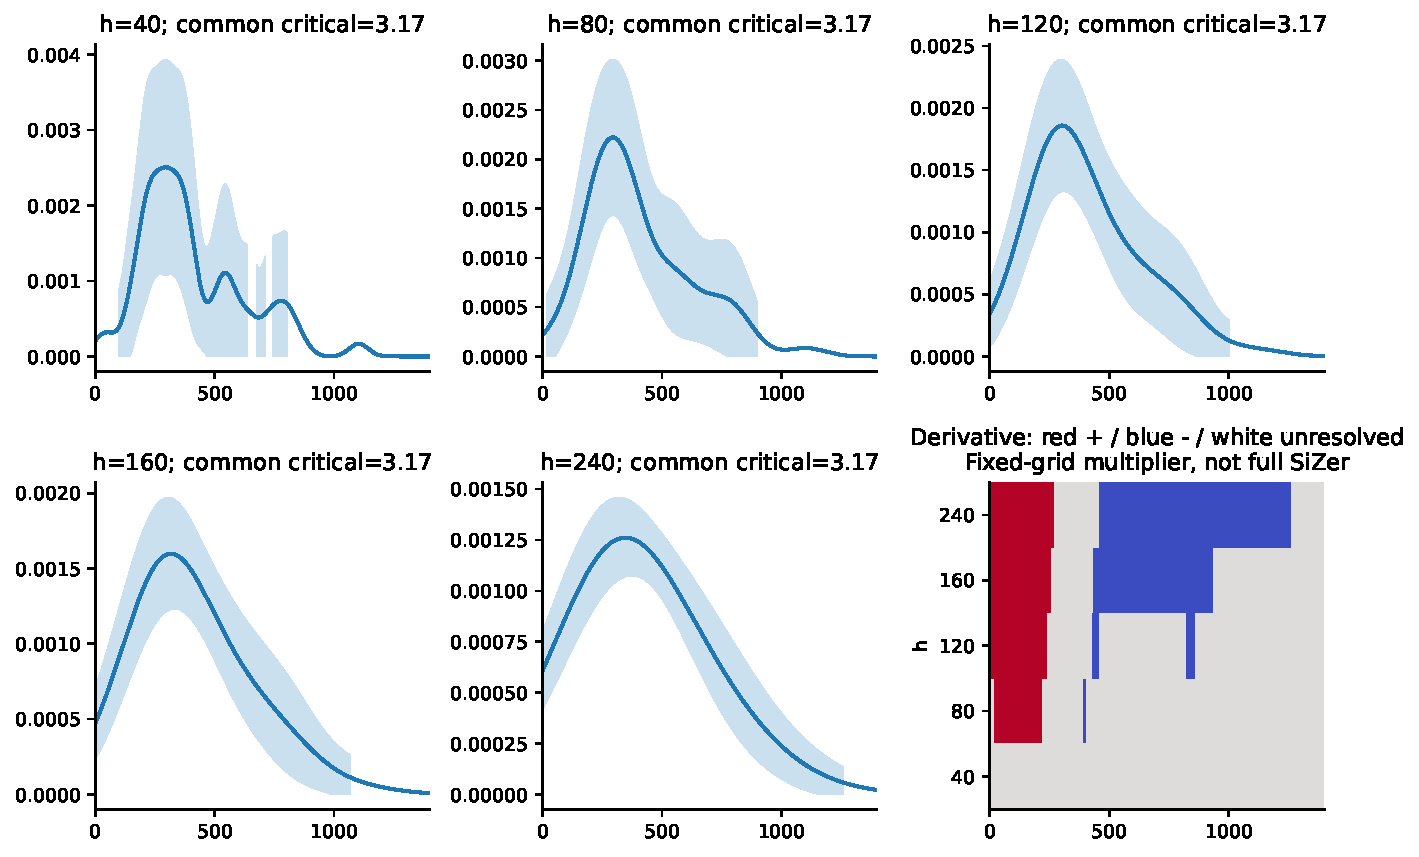
\includegraphics[width=\linewidth]{kde_computation/figures/ceo_bands.pdf}\end{center}
\begin{center}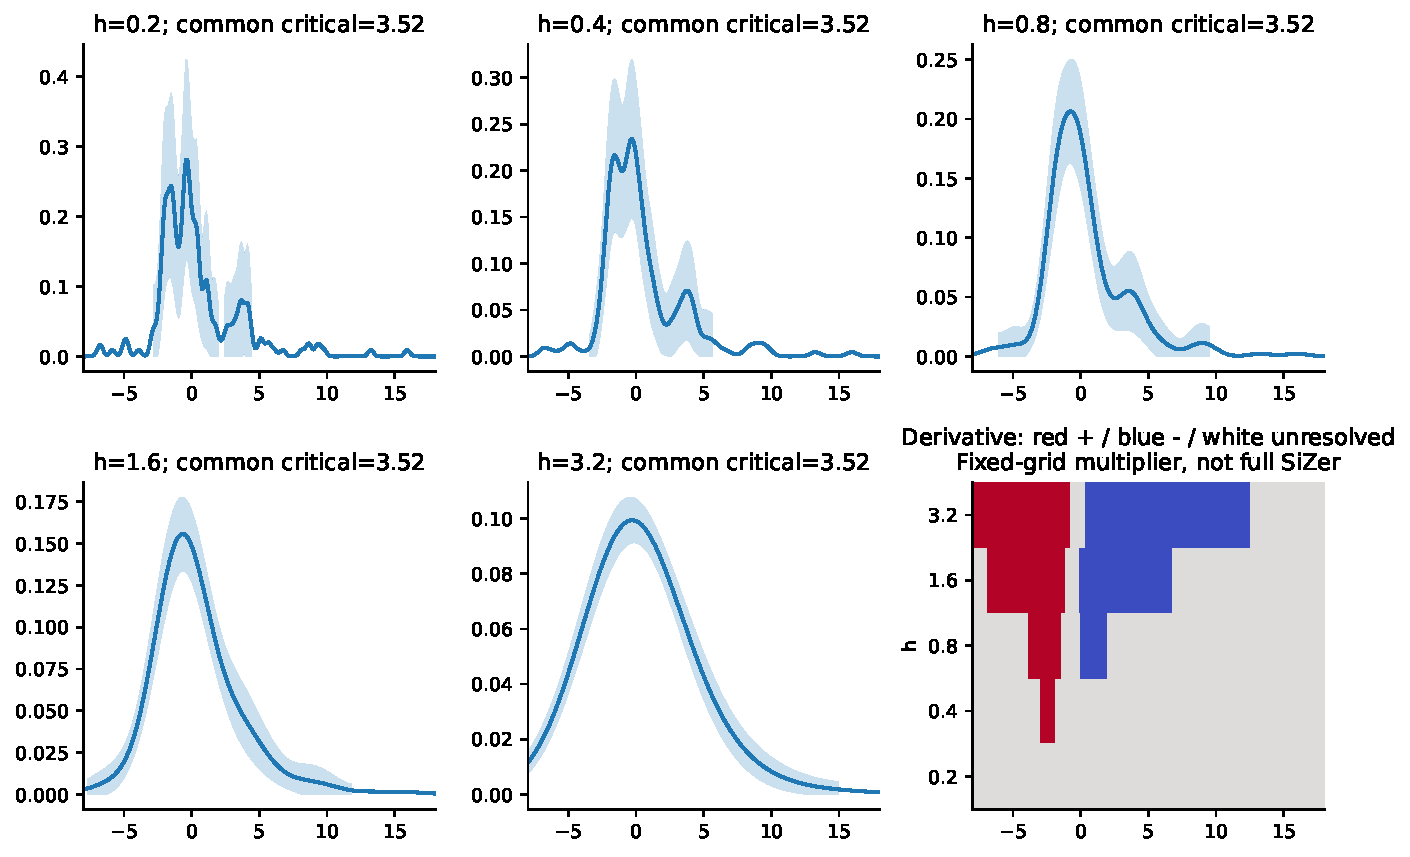
\includegraphics[width=\linewidth]{kde_computation/figures/glass_bands.pdf}\end{center}

CEO còn có biên tự nhiên $0$. Gaussian KDE trên toàn trục có thể đặt khối lượng lên vùng âm. Nếu mục tiêu là mật độ sát 0, cân nhắc phản xạ hoặc ước lượng trên $\log X$, rồi đổi ngược $\widehat f_X(x)=\widehat f_{\log X}(\log x)/x$; các hình trên giữ KDE gốc để so đúng yêu cầu của đề.
\par\textbf{Viết nhanh:} CEO dùng $n=59$, $h_{NR}=101.32$, $h_{CV}=69.45$; glass dùng $n=214$, $h_{NR}=0.7127$, $h_{CV}=0.2393$. CV giữ nhiều gợn hơn; các gợn nhỏ chưa được xác nhận bằng băng đạo hàm. Phân biệt $f_h$, trung bình trên bin và $f$ thật.
\end{solution}

\begin{problem}[KDE-42. W6.9: local polynomial density trên glass, có công thức tính trực tiếp.]\label{k:42}
\textit{(Nguồn: W mục 6.4, W6.9, tr.143.)} Tính local likelihood bậc $p=0,1,2$ và so sánh với KDE trên cùng dữ liệu glass.
\end{problem}
\begin{solution}
\textbf{1. Bài toán tối ưu.} Với $t_i=X_i-x$, $w_i=\phi(t_i/h)$ và $P(t)=a_0+a_1t+a_2t^2/2$, cực đại
\[
 L_x(a)=\sum_iw_iP(t_i)-n\int_{\R}\phi(t/h)e^{P(t)}dt.
\]
Ở đây tích phân trên toàn $\R$, không cắt nhân Gaussian tại $[-1,1]$.
Đặt $S=\sum_iw_i$, $m=\sum_iw_it_i/S$, $v=\sum_iw_i(t_i-m)^2/S$.

\textbf{2. Bậc 0.} Vì $\int\phi(t/h)dt=h$, phương trình đạo hàm là $S-nhe^{a_0}=0$; suy ra
$e^{a_0}=S/(nh)=\widehat f_h(x)$, đúng KDE-38. Code đã đối chiếu hai cách tính.

\textbf{3. Bậc 1.} Hoàn bình phương cho
\[
 \int\phi(t/h)e^{a_0+a_1t}dt
 =h\exp(a_0+h^2a_1^2/2).
\]
Các phương trình score cho tổng khối lượng và moment bậc 1 cho $h^2a_1=m$ và $nhe^{a_0+h^2a_1^2/2}=S$. Vậy
\[
 \widehat a_1=m/h^2,\qquad
 \widehat f_{LL,1}(x)=\frac{S}{nh}\exp\{-m^2/(2h^2)\}.
\]
Trước chuẩn hóa, đường này không vượt KDE tại cùng $x,h$. Điều đó \emph{không} có nghĩa bias hoặc MISE luôn nhỏ hơn.

\textbf{4. Bậc 2.} Điều kiện tích phân hữu hạn là $a_2<h^{-2}$.
Mật độ chuẩn tỷ lệ với $\phi(t/h)e^{P(t)}$ có phương sai $V=(h^{-2}-a_2)^{-1}$ và trung bình $a_1V$.
Ba phương trình score khớp tổng, moment 1 và moment 2, nên $V=v$, $a_1V=m$ và
\[
 \boxed{\widehat a_2=h^{-2}-v^{-1},\quad
 \widehat a_1=m/v,\quad
 \widehat f_{LL,2}(x)=\frac{S}{n\sqrt v}\exp\{-m^2/(2v)\}.}
\]
Điều kiện là $S>0,v>0$; khi các trọng số tập trung gần một quan sát, $v$ rất nhỏ, nghiệm có thể mất ổn định. Tính lõm của log-likelihood không tự bảo đảm mọi bước Newton hội tụ hoặc mọi dữ liệu có nghiệm tốt. Công thức đóng tránh vòng tối ưu số ở ví dụ Gaussian này.

\textbf{5. Kết quả thực nghiệm.} Để tách hiệu ứng bậc đa thức, dùng chung hai bandwidth đã có: $h_{CV}=0.23925$ và $h_{NR}=0.71269$, không tuyên bố chúng tối ưu riêng cho local likelihood.
Các đường local likelihood dương nhưng nhìn chung không tích phân bằng 1. Trên lưới 501 điểm $[-8,18]$, tích phân thô của bậc $0,1,2$ lần lượt xấp xỉ
\[
 \begin{array}{c|ccc}
  &p=0&p=1&p=2\\\hline
 h_{CV}&1.00000&0.95707&1.01279\\
 h_{NR}&0.99958&0.91881&1.01220
 \end{array}
\]
Đồ thị chia từng đường cho tích phân số trên miền này để so các mật độ có cùng khối lượng trên miền. Đây là bước hậu xử lý, khác định nghĩa thô $e^{\widehat a_0}$ trong sách; riêng KDE Gaussian vốn có tổng khối lượng 1 trên toàn trục.
\begin{center}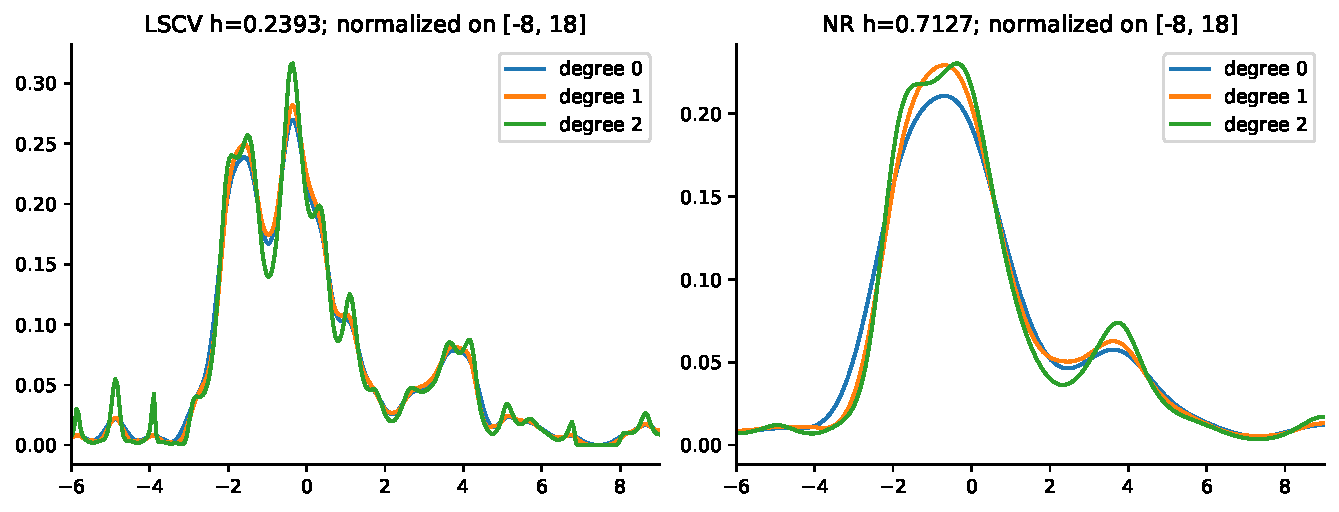
\includegraphics[width=\linewidth]{kde_computation/figures/glass_local_likelihood.pdf}\end{center}
Với $h_{CV}$, mật độ cực đại sau chuẩn hóa của $p=0,1,2$ lần lượt khoảng $0.2698,0.2819,0.3164$: bậc 2 tạo đỉnh sắc hơn. Với $h_{NR}$, các cực đại khoảng $0.2108,0.2293,0.2304$ và các đường trơn hơn. Vì không biết $f$ thật của glass, không thể từ hình này kết luận bậc 2 có ISE nhỏ nhất. Việc xử lý một biên đã biết cần thay miền tích phân trong local likelihood; không dùng các công thức toàn trục này như một chứng minh tự động sửa mọi bias biên.
\par\textbf{Viết nhanh:} Đặt $S,m,v$ là tổng và moment có trọng số Gaussian. Bậc 0: $S/(nh)$; bậc 1: $S e^{-m^2/(2h^2)}/(nh)$; bậc 2: $S e^{-m^2/(2v)}/(n\sqrt v)$. Local likelihood dương nhưng cần kiểm tra chuẩn hóa và ổn định.
\end{solution}

\begin{problem}[KDE-43. W6.10: Bart Simpson, KDE so với chuyển sang hồi quy.]\label{k:43}
\textit{(Nguồn: W6.10, tr.144; W (6.2) và mục 6.6.)} Sinh mẫu ở $n=25,50,100,1000$; tính KDE và phương pháp chuyển mật độ thành hồi quy, so sánh bằng hình và ISE.
\end{problem}
\begin{solution}
\textbf{1. Sinh đúng hỗn hợp.} Mật độ thật là
\[
 f(x)=\tfrac12\phi(x)+\tfrac1{10}\sum_{j=0}^4
 \frac1{0.1}\phi\!\left(\frac{x-(j/2-1)}{0.1}\right).
\]
Với xác suất $1/2$, sinh $N(0,1)$; nếu không, chọn đều $j\in\{0,\ldots,4\}$ rồi sinh $N(j/2-1,0.1^2)$.
$0.1$ là \emph{độ lệch chuẩn}, không phải phương sai; mỗi móng có trọng số $0.1$ và tổng trọng số bằng 1.
Do đối xứng, $\E X=0$ và
\[
 \Var X=0.5+0.1\sum_{j=0}^4[0.01+(j/2-1)^2]=0.755.
\]
Thang toàn cục $\sqrt{0.755}\approx0.869$ lớn hơn nhiều bề rộng $0.1$ của mỗi móng: đây là lý do normal reference dễ làm mờ móng.

\textbf{2. KDE.} Trong mỗi mẫu, tính riêng $h_{NR}$, $h_{CV}$ theo thuật toán KDE-41, rồi đánh giá hai KDE Gaussian. Không dùng $f$ thật để chọn bandwidth; $f$ thật chỉ dùng chấm ISE.

\textbf{3. Chuyển thành hồi quy đúng đơn vị.}
Chọn miền cố định $[a,b]=[-6,6]$, chia $k=\max(3,\lfloor n/10+1/2\rfloor)$ bin; vì thế $k=3,5,10,100$.
Đặt $\Delta=12/k$, $t_j$ là trung điểm và
\[
 Y_j=\sqrt{\frac{N_j+1/4}{n\Delta}},\qquad
 \E Y_j\approx\sqrt{f(t_j)},\qquad
 \Var Y_j\approx\frac1{4n\Delta}.
\]
Đây là công thức (6.49) sau đổi biến từ $[0,1]$ về $[a,b]$; bỏ mất $\Delta$ sẽ sai đơn vị mật độ. Xấp xỉ dùng Poisson hóa và delta method, kém ở bin thưa. Count thật có phân phối multinomial nên không hoàn toàn độc lập.

Dùng hồi quy kernel hằng cục bộ:
\[
 \widehat r_b(x)=\frac{\sum_j\phi((x-t_j)/b)Y_j}{\sum_j\phi((x-t_j)/b)},\qquad
 \widehat{\boldsymbol Y}=S_b\boldsymbol Y.
\]
Ở đây $b$ trong $\widehat r_b$ ký hiệu bandwidth hồi quy, không phải cận phải của miền.
Chọn bandwidth bằng
\[
 \operatorname{GCV}(b)=\frac{k^{-1}\|Y-S_bY\|^2}{(1-\operatorname{tr}(S_b)/k)^2}
\]
trên 61 điểm log từ $0.25\Delta$ đến $4$. Sau đó lấy
\[
 \widehat f_{reg}(x)=\frac{\max(\widehat r_b(x),0)^2}
 {\int_{-6}^{6}\max(\widehat r_b(u),0)^2du},\quad x\in[-6,6],
\]
và đặt 0 ngoài miền. Phương pháp mục 6.6 cho phép chọn phương pháp hồi quy; đây là một triển khai cụ thể bằng kernel regression và GCV, không phải kết quả chung cho mọi cách hồi quy.

\textbf{4. Tiêu chí chấm và kết quả.}
Chạy $40$ mẫu độc lập cho mỗi $n$; tính ISE trên 2401 điểm đều của $[-6,6]$ (bước $0.005$). Miền này bỏ qua đuôi Gaussian rất nhỏ; không cắt hay bỏ bất cứ quan sát nào trong các lần chạy. Hình vẽ mẫu đầu tiên, không lựa mẫu đẹp nhất.
Bảng là trung bình ISE $\pm$ \emph{một sai số chuẩn Monte Carlo}, với
$\mathrm{MCSE}=s(\mathrm{ISE}_1,\ldots,\mathrm{ISE}_{40})/\sqrt{40}$.
Đây không phải khoảng tin cậy 95\% và trung bình thực nghiệm chỉ xấp xỉ MISE.
\begin{center}\small\begin{tabular}{rrrr}\toprule $n$ & KDE NR & KDE CV & Mục 6.6 (GCV)\\\midrule
25 & $0.0744 \pm 0.0036$ & $0.1045 \pm 0.0124$ & $0.2489 \pm 0.0007$\\
50 & $0.0563 \pm 0.0010$ & $0.0701 \pm 0.0053$ & $0.1284 \pm 0.0074$\\
100 & $0.0530 \pm 0.0008$ & $0.0471 \pm 0.0034$ & $0.0529 \pm 0.0004$\\
1000 & $0.0429 \pm 0.0001$ & $0.0072 \pm 0.0004$ & $0.0084 \pm 0.0003$\\
\bottomrule\end{tabular}\end{center}
\begin{center}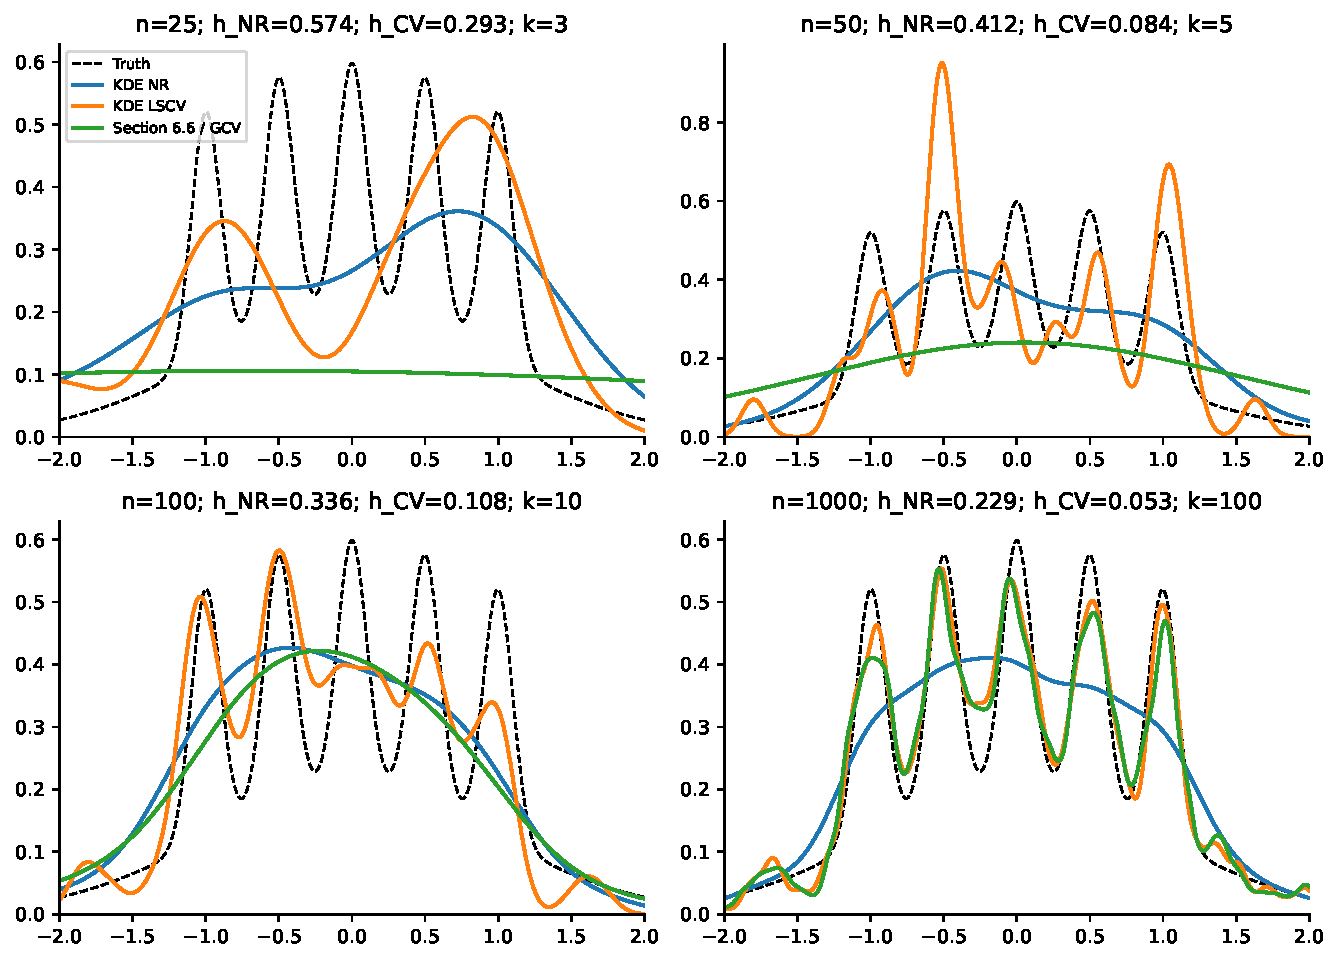
\includegraphics[width=\linewidth]{kde_computation/figures/bart_comparison.pdf}\end{center}

\textbf{5. Diễn giải để viết vào bài.}
Ở $n=25,50$, CV có trung bình ISE lớn hơn NR trong thí nghiệm này: biến thiên do chọn bandwidth lớn có thể lấn át lợi ích giảm bias. Không được viết ``CV luôn tốt hơn''.
Ở $n=1000$, ISE trung bình của NR khoảng $0.0429$, CV $0.00723$, hồi quy $0.00838$: hai phương pháp sau phân giải móng tốt hơn. Bandwidth CV trung bình khoảng $0.0512$, NR khoảng $0.2322$, phù hợp với bề rộng móng.

Với $n=25$ chỉ có ba bin, mỗi bin rộng $4$: thông tin về năm móng đã mất trong phép gộp bin; GCV không thể tái tạo chi tiết không còn trong counts. Cực tiểu GCV nằm ở đầu mút lưới trong $40/40$ lần với $n=25$ và $5/40$ lần với $n=50$, nhưng không lần nào với $n=100,1000$. Vì vậy các kết quả mẫu nhỏ của hồi quy đặc biệt nhạy với cách chia bin, miền và lưới bandwidth, không phải bằng chứng phương pháp 6.6 nói chung kém.
Ở $n=1000$, bin rộng $0.12$ vẫn gây làm trơn trước khi hồi quy; miền ngắn hơn hoặc nhiều bin hơn có thể đổi so sánh. Phải công bố lựa chọn này thay vì quy mọi khác biệt cho KDE hay hồi quy.

\par\textbf{Viết nhanh:} Sinh hỗn hợp với SD móng $0.1$; chuyển count thành $Y_j=\sqrt{(N_j+1/4)/(n\Delta)}$, hồi quy rồi bình phương và chuẩn hóa. NR dễ làm mất móng; CV dao động ở mẫu nhỏ, tốt hơn rõ trong thí nghiệm $n=1000$. So bằng ISE khi biết $f$, công bố cả MCSE.
\end{solution}

\nhom{Ghi chú tái lập phần tính toán}
\noindent Trong thư mục \texttt{kde\_computation} có dữ liệu, mã, tám đồ thị PDF, các ISE từng lần mô phỏng, hai bảng \LaTeX{} và \texttt{results.json} lưu seed, phiên bản thư viện và SHA-256 của dữ liệu. Chạy từ thư mục Exercise:
\begin{verbatim}
OPENBLAS_NUM_THREADS=1 OMP_NUM_THREADS=1 \
python kde_computation/run_kde_experiments.py
latexmk -xelatex -interaction=nonstopmode \
  -halt-on-error KDE_Exam_Complete_Solutions.tex
\end{verbatim}
Mã tự kiểm tra chuẩn hóa nhân, CV theo tổng cặp so với định nghĩa leave-one-out và tích phân số, cùng đẳng thức local likelihood bậc 0 = KDE. Các lựa chọn lưới, miền tích phân và băng tin cậy được ghi rõ để đáp số có thể đối chiếu.
